% A-appendix.tex
% ---------------------------

\section{APPENDIX} \label{sec:appendix}

    % Images:
    % images/maps/Monte_Cappuccini.png
    % images/maps/Tram_15_trip_Castello_to_Pescatore.png
    % images/screenshots/Screenshot_20250503_GnssLogger_map.jpg
    % images/screenshots/Screenshot_20250503_GnssLogger_plots.jpg
    % images/screenshots/Screenshot_20250503_GnssLogger_spoof_jam.jpg
    % images/screenshots/Screenshot_20250503_GnssLogger_status.jpg
    % images/screenshots/Screenshot_20250503_GnssLogger_measurements.jpg
    % images/screenshots/Screenshot_20250503_GnssLogger_skyplot.jpg

    \subsection{GNSS Logger Screenshots}

        \noindent The following figures show screenshots from the GNSS Logger app, illustrating various features and data visualizations available during the GNSS data collection process of the \textit{Monte dei Cappuccini} test.

        \begin{figure}[htbp]
            \centering
            \begin{subfigure}{0.23\textwidth}
                \centering
                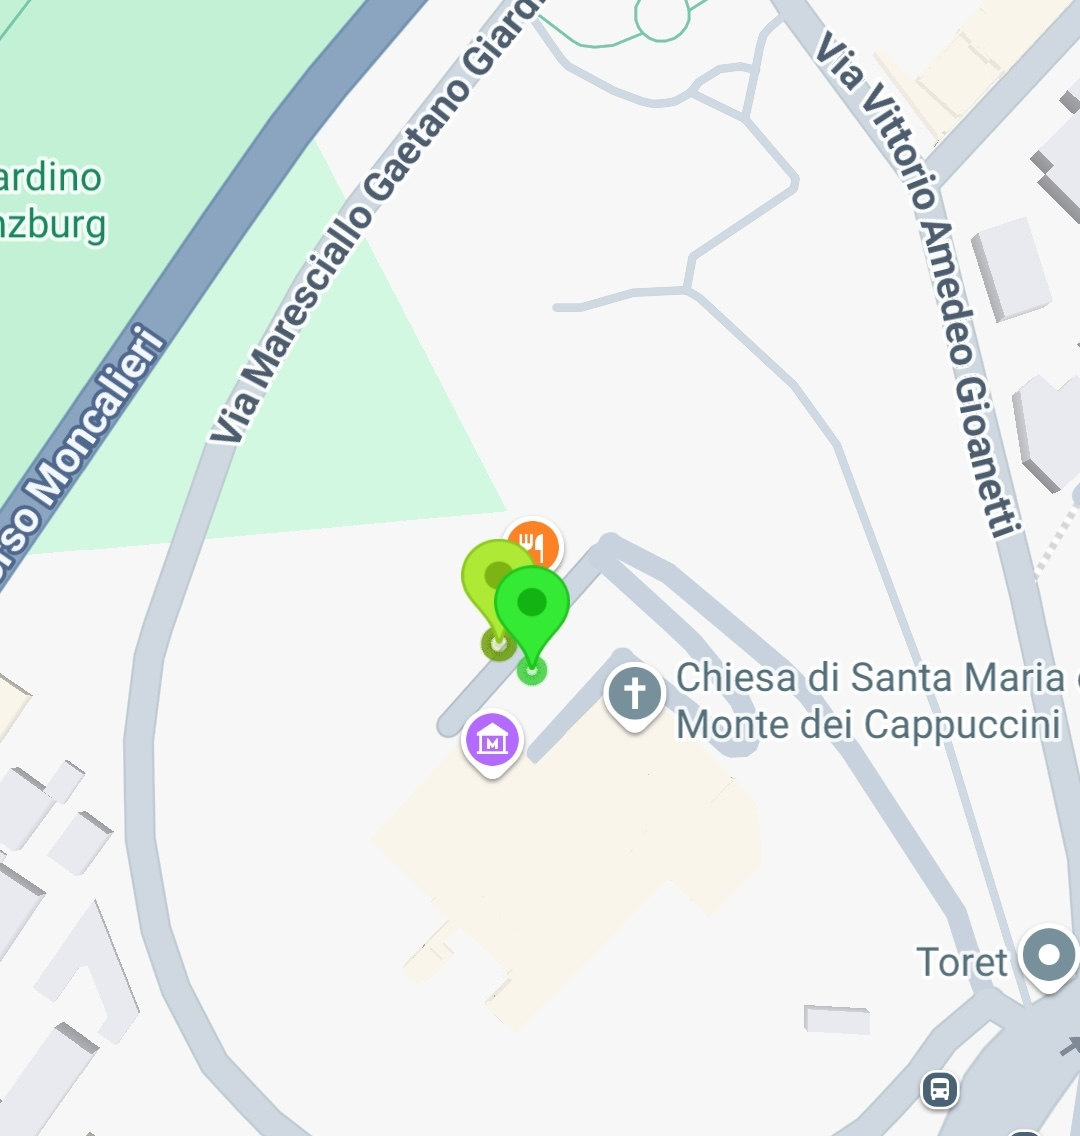
\includegraphics[width=\textwidth]{images/screenshots/Screenshot_20250503_GnssLogger_map.jpg}
                \caption{Monte dei Cappuccini Map}
                \label{fig:gnsslogger_map}
            \end{subfigure}
            \hfill
            \begin{subfigure}{0.23\textwidth}
                \centering
                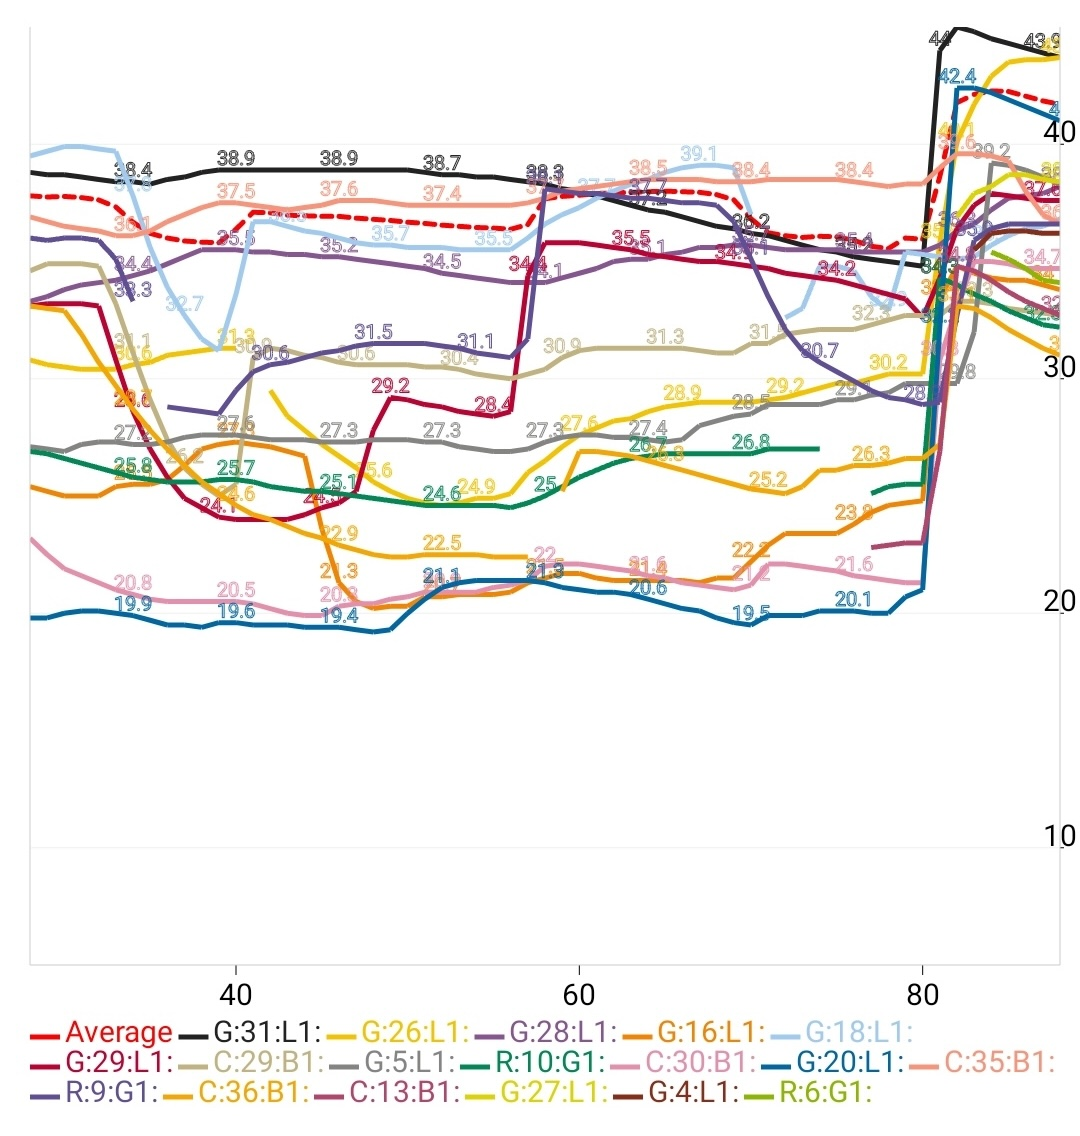
\includegraphics[width=\textwidth]{images/screenshots/Screenshot_20250503_GnssLogger_plots.jpg}
                \caption{CN0(db.Hz) vs Time(s)}
                \label{fig:gnsslogger_plots}
            \end{subfigure}
            \vspace{0.35cm}
            \caption{GNSS Logger Map (a) and Plots (b).}
            \label{fig:gnsslogger_1}
        \end{figure}

        \vspace{0.1cm}

        \begin{figure}[htbp]
            \centering
            \begin{subfigure}{0.23\textwidth}
                \centering
                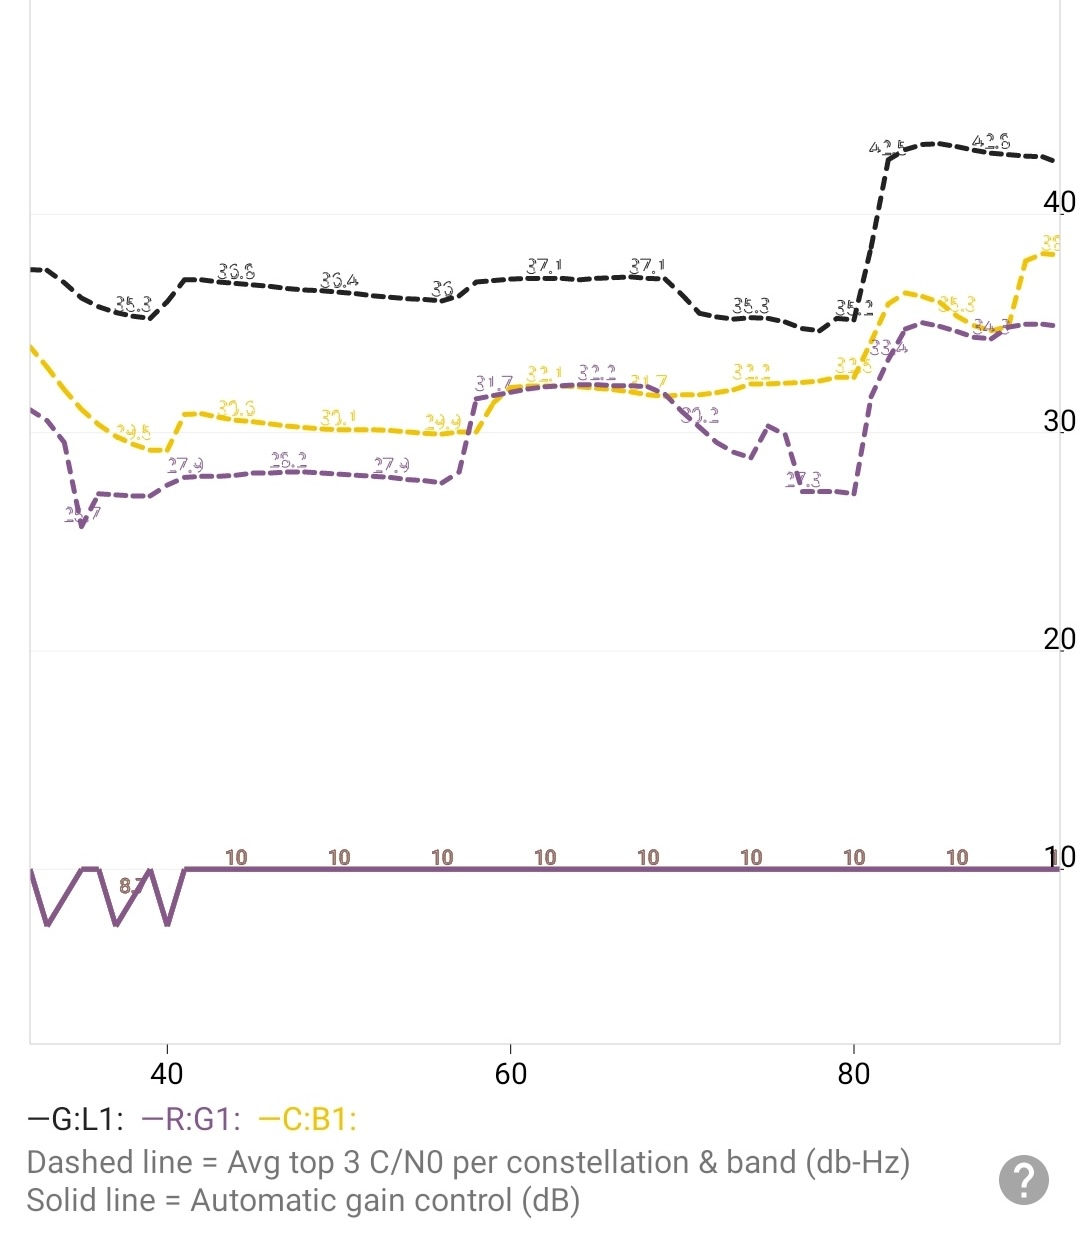
\includegraphics[width=\textwidth]{images/screenshots/Screenshot_20250503_GnssLogger_spoof_jam.jpg}
                \caption{Auto gain control \& C/N0 vs (s)}
                \label{fig:gnsslogger_spoof_jam}
            \end{subfigure}
            \hfill
            \begin{subfigure}{0.23\textwidth}
                \centering
                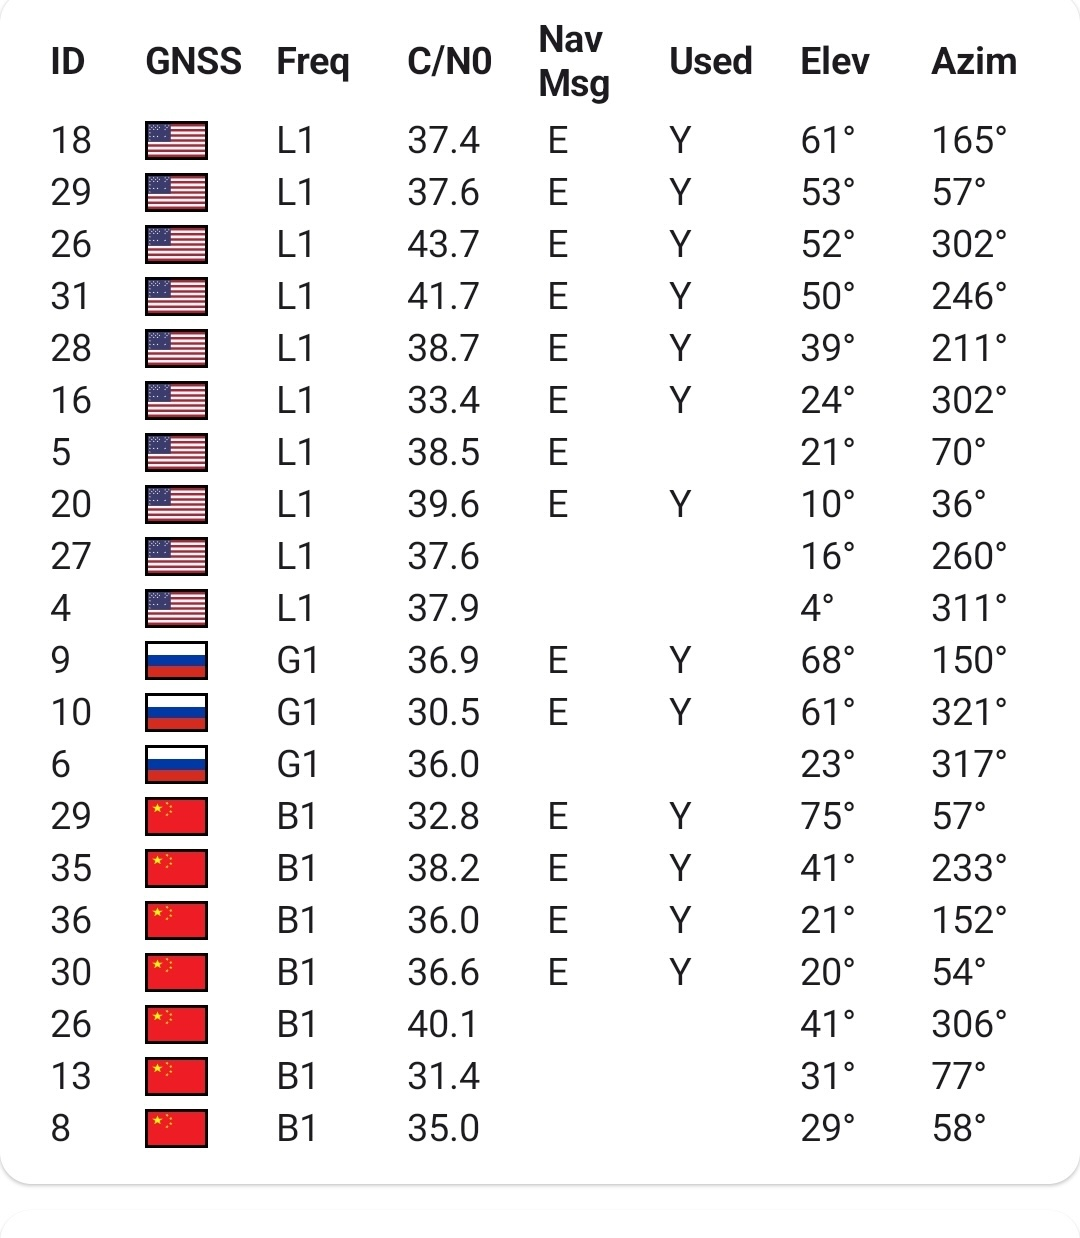
\includegraphics[width=\textwidth]{images/screenshots/Screenshot_20250503_GnssLogger_status.jpg}
                \caption{[SBAS satellites not available]}
                \label{fig:gnsslogger_status}
            \end{subfigure}
            \vspace{0.35cm}
            \caption{GNSS Logger Spoof/Jam (a) and Status (b).}
            \label{fig:gnsslogger_2}
        \end{figure}

        \vspace{0.1cm}

        \begin{figure}[htbp]
            \centering
            \begin{subfigure}{0.23\textwidth}
                \centering
                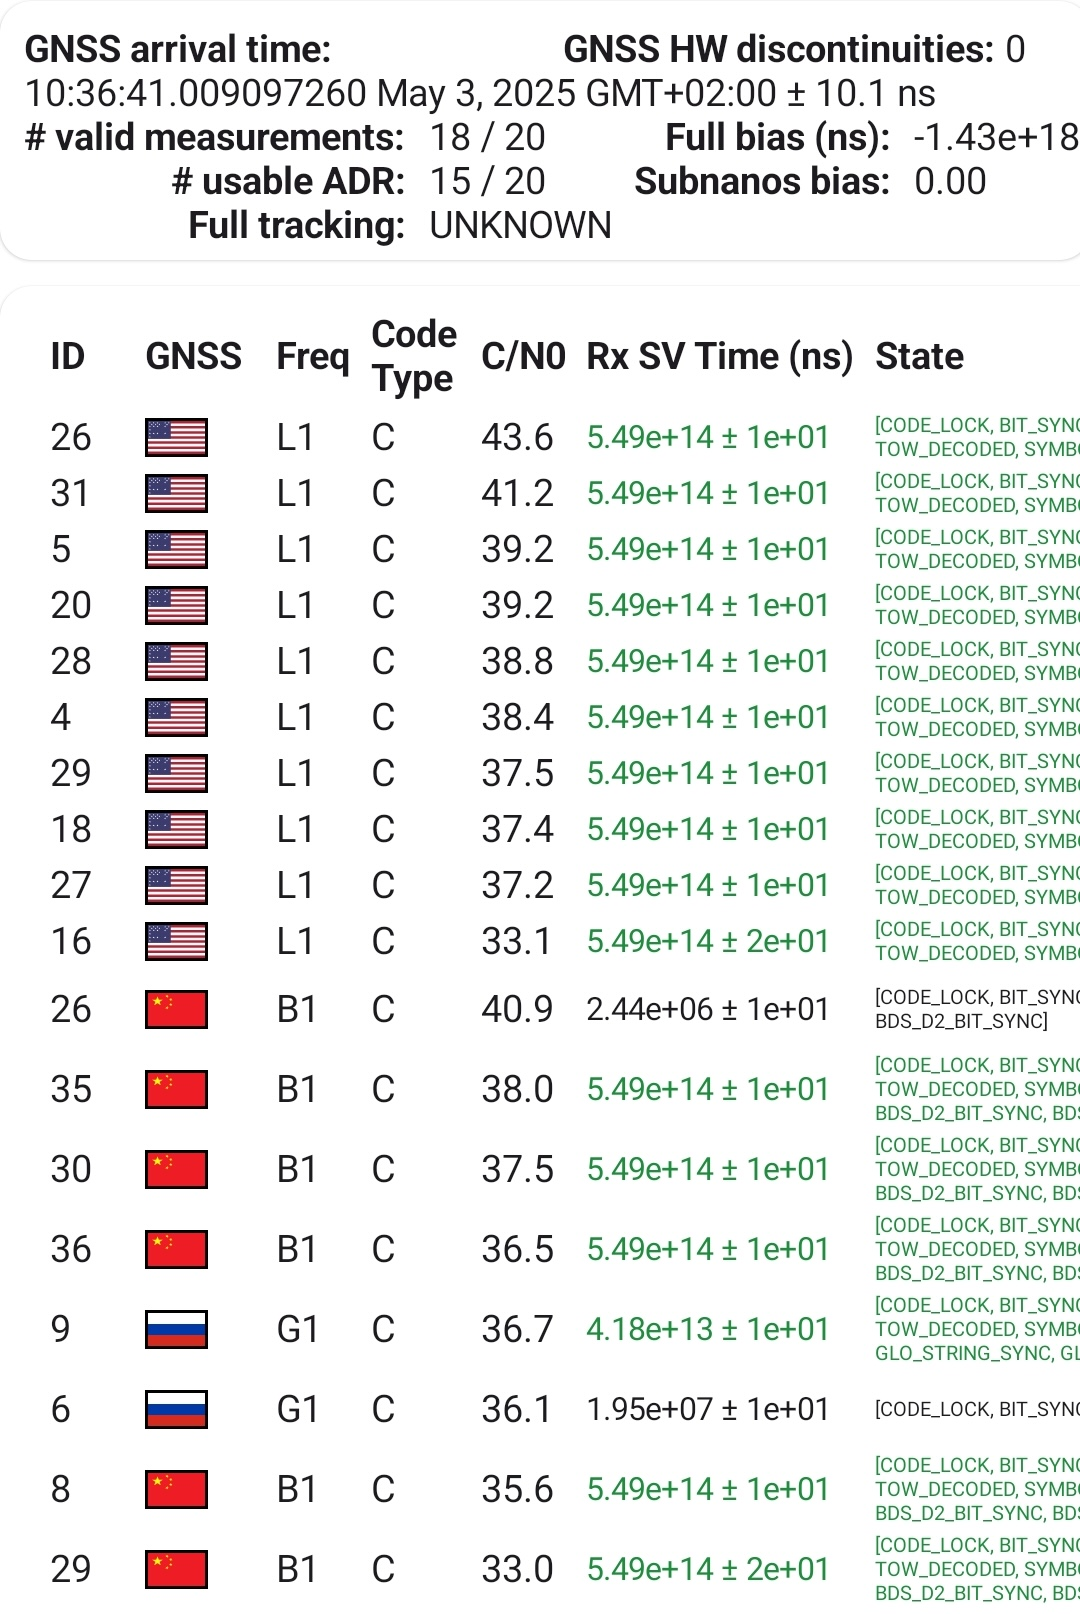
\includegraphics[width=\textwidth]{images/screenshots/Screenshot_20250503_GnssLogger_measurements.jpg}
                % \caption{}
                \label{fig:gnsslogger_measurements}
            \end{subfigure}
            \hfill
            \begin{subfigure}{0.23\textwidth}
                \centering
                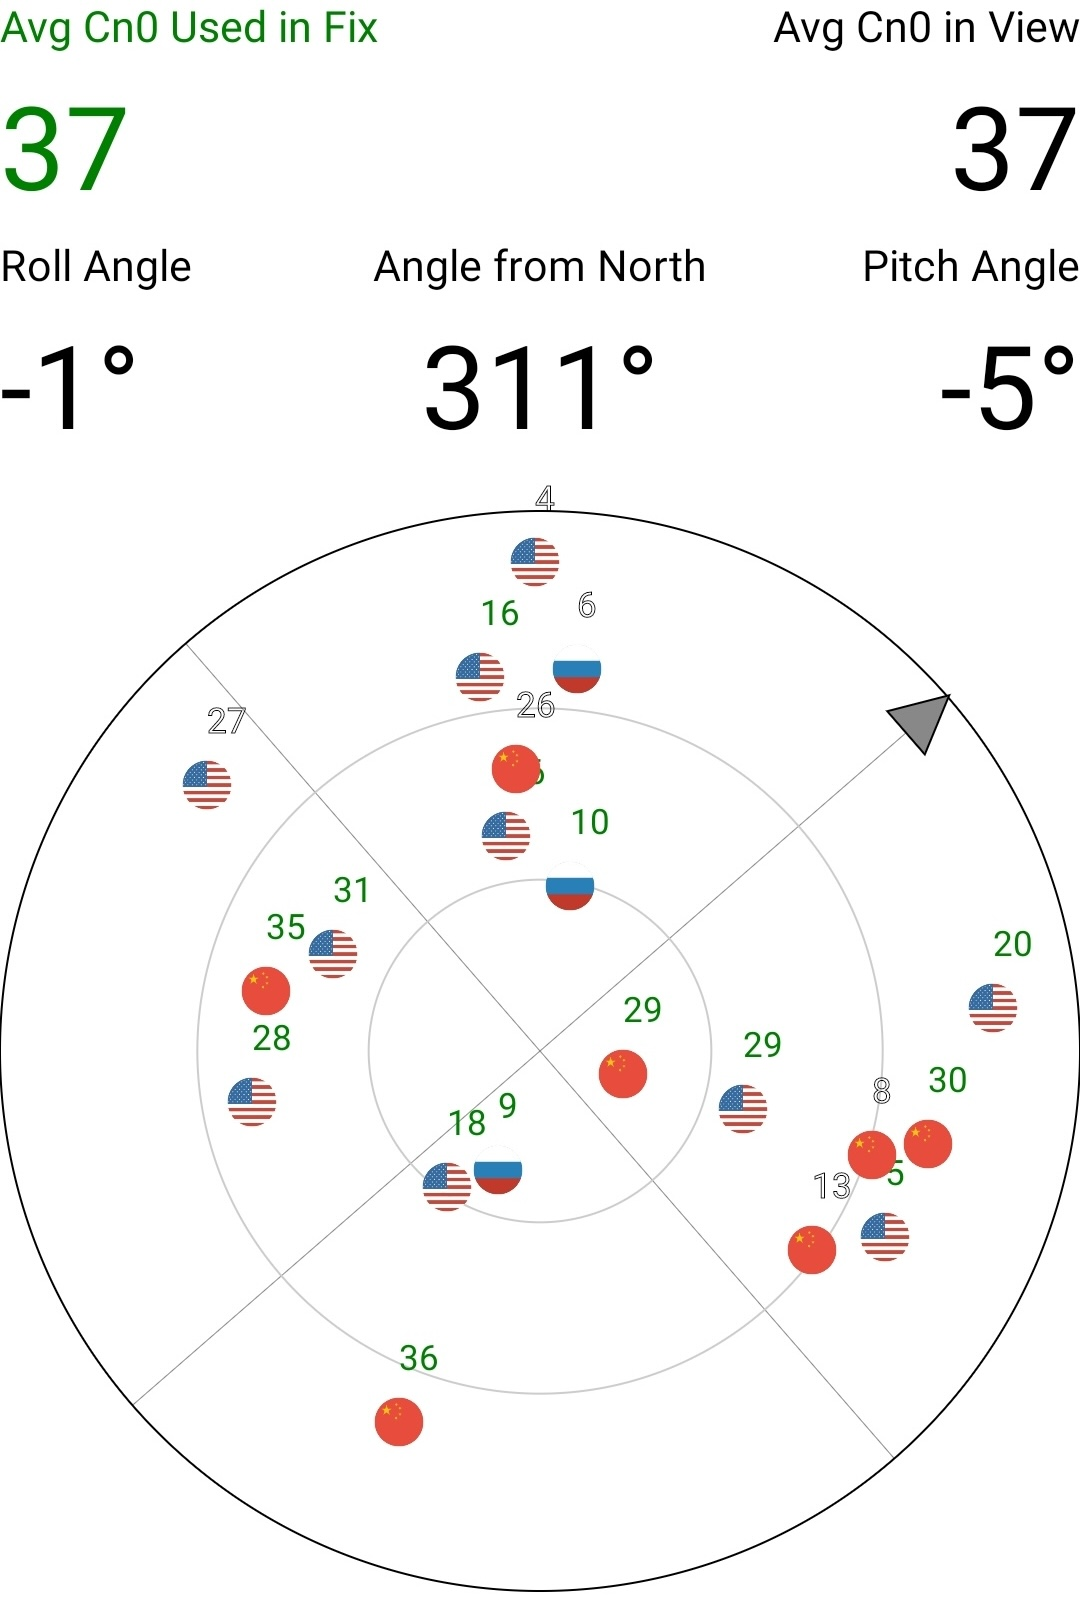
\includegraphics[width=\textwidth]{images/screenshots/Screenshot_20250503_GnssLogger_skyplot.jpg}
                % \caption{}
                \label{fig:gnsslogger_skyplot}
            \end{subfigure}
            % \vspace{0.35cm}
            \caption{GNSS Logger Measurements (a) and Skyplot (b).}
            \label{fig:gnsslogger_3}
        \end{figure}
